\chapter{Marco Teórico}

\section{Medidas de tendencia central}

Las medidas de tendencia central son herramientas estadísticas que nos permiten resumir la localización de los datos, es decir, nos ayudan a identificar el valor alrededor del cual se centran los datos. Estas medidas son esenciales para el análisis de datos en cualquier investigación, incluyendo el análisis de las muestras de Lengua de Señas Mexicana (LSM).

\textbf{Medidas de tendencia central:}

\textbf{Media:}

La media aritmética es el valor obtenido al sumar todos los valores de un conjunto de datos y dividir entre el número de datos. En el análisis de LSM, la media puede utilizarse para calcular la posición promedio de las manos en una seña.

\indexedequation{Media aritmética}{
\begin{equation}
    \bar{x} = \frac{\sum_{i=1}^{n} x_i}{n}
    \label{eq:media}
\end{equation}
}


\textbf{Varianza:}

La varianza es una medida de dispersión que indica cuánto varían los datos alrededor de la media. Una varianza alta indica que los datos están más dispersos, mientras que una varianza baja indica que los datos están más agrupados alrededor de la media.

La fórmula para calcular la varianza es:
\indexedequation{Varianza}{
    \begin{equation}
        \sigma^2 = \frac{\sum_{i=1}^{n} (x_i - \bar{x})^2}{n-1}
        \label{eq:varianza}
    \end{equation}
}


\textbf{Desviación Estándar:}

La desviación estándar es una medida de dispersión que indica cuánto varían los datos alrededor de la media. Una desviación estándar alta indica que los datos están más dispersos, mientras que una desviación estándar baja indica que los datos están más agrupados alrededor de la media.

La fórmula para calcular la desviación estándar es:
\indexedequation{Desviación estándar}{
\begin{equation}
    \sigma = \sqrt{\frac{\sum_{i=1}^{n} (x_i - \bar{x})^2}{n-1}}
    \label{eq:desviacion_estandar}
\end{equation}
}

\section{MediaPipe Holistic}

MediaPipe Holistic es una solución integral de Google para el seguimiento del cuerpo humano en tiempo real. El modelo de Holistic combina  modelos de aprendizaje profundo para detectar y rastrear puntos (posiciones flotantes en un  plano x, y) clave en el rostro, las manos y el cuerpo completo. Esta capacidad de análisis detallado de los movimientos corporales es esencial para la captura expresiva de la Lengua de Señas Mexicana (LSM), donde la posición del cuerpo y los movimientos de las manos son fundamentales para recibir y generar la comunicación.

\subsection{Componentes del Modelo Holistic}

MediaPipe Holistic se compone de tres modelos principales:

\begin{enumerate}
    \item \textbf{Pose Landmarker:}
    \begin{itemize}
        \item \textbf{Descripción:}  Este modelo detecta 33 puntos de referencia del cuerpo humano en una imagen o video, incluyendo la nariz, los ojos, las orejas, los hombros, los codos, las muñecas, las caderas, las rodillas y los tobillos. 
        \item \textbf{Aplicaciones en lengua de señas mexicana:}  Estos puntos son cruciales para interpretar las señas, ya que permiten analizar la postura general del cuerpo y la posición de los brazos y las manos en relación al torso. Por ejemplo, la posición de los codos y las muñecas es fundamental para distinguir señas como \textquotedblleft CASA\textquotedblright  u  \textquotedblleft HOLA\textquotedblright.
        \item \textbf{Funcionamiento:} El modelo utiliza una red neuronal convolucional similar a MobileNetV2 y está optimizado para aplicaciones de entrenamiento en tiempo real y en el dispositivo.  Primero, detecta la presencia de cuerpos humanos en la imagen, y luego localiza los 33 puntos de referencia en el cuerpo detectado.
        \item \textbf{Opciones de configuración:}  
            \begin{itemize}
                \item \textbf{running\_mode:} Establece el modo de ejecución (IMAGE, VIDEO, LIVE\_STREAM).
                \item \textbf{num\_poses:} La cantidad máxima de poses a detectar.
                \item \textbf{min\_pose\_detection\_confidence:} Puntuación mínima para la detección de poses.
                \item \textbf{min\_pose\_presence\_confidence:} Puntuación mínima de presencia de poses.
                \item \textbf{min\_tracking\_confidence:} Puntuación mínima para el seguimiento de poses.
                \item \textbf{output\_segmentation\_masks:}  Si se generan máscaras de segmentación.
            \end{itemize}
    \end{itemize}
    \begin{figure}[h]
        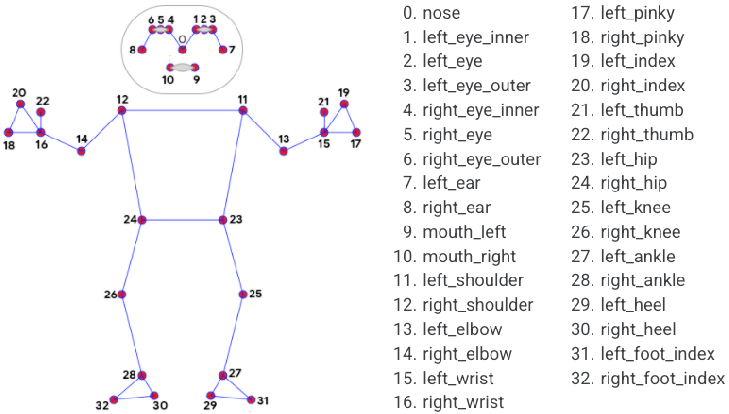
\includegraphics[scale=0.4]{CAPITULOS/capitulo2/img.png}
        \centering
        \caption[Puntos de medipipe]{Puntos de medipipe Pose Landmarker \cite{ref20}}
        \label{fig:imagen_medipipe_pose}
    \end{figure}
    \item \textbf{Face Landmarks:}
    \begin{itemize}
        \item \textbf{Cantidad:} 468 puntos.
        \item \textbf{Descripción:}  Detecta puntos clave en el rostro, como los ojos, las cejas, la nariz, la boca y el contorno de la cara.
        \item \textbf{Aplicaciones de MediaPipe Holistic en el sistema:} Se utilizan para analizar las expresiones faciales, que son un componente gramatical crucial en la LSM. Por ejemplo, las expresiones faciales pueden indicar preguntas, negación, o emociones.
    \end{itemize}

    \item \textbf{Hand Landmarks:}
    \begin{itemize}
        \item \textbf{Cantidad:} 21 puntos por cada mano \cite{ref20}.
        \item \textbf{Descripción:} Detecta  puntos clave en las manos, como las puntas de los dedos, los nudillos y la palma.
        \item \textbf{Aplicaciones de MediaPipe Holistic en el sistema:} Permite analizar la forma, orientación y movimiento de las manos, lo cual es fundamental para identificar los diferentes queremas (formas de la mano) en la LSM.
    \end{itemize}
    \begin{figure}[h]
              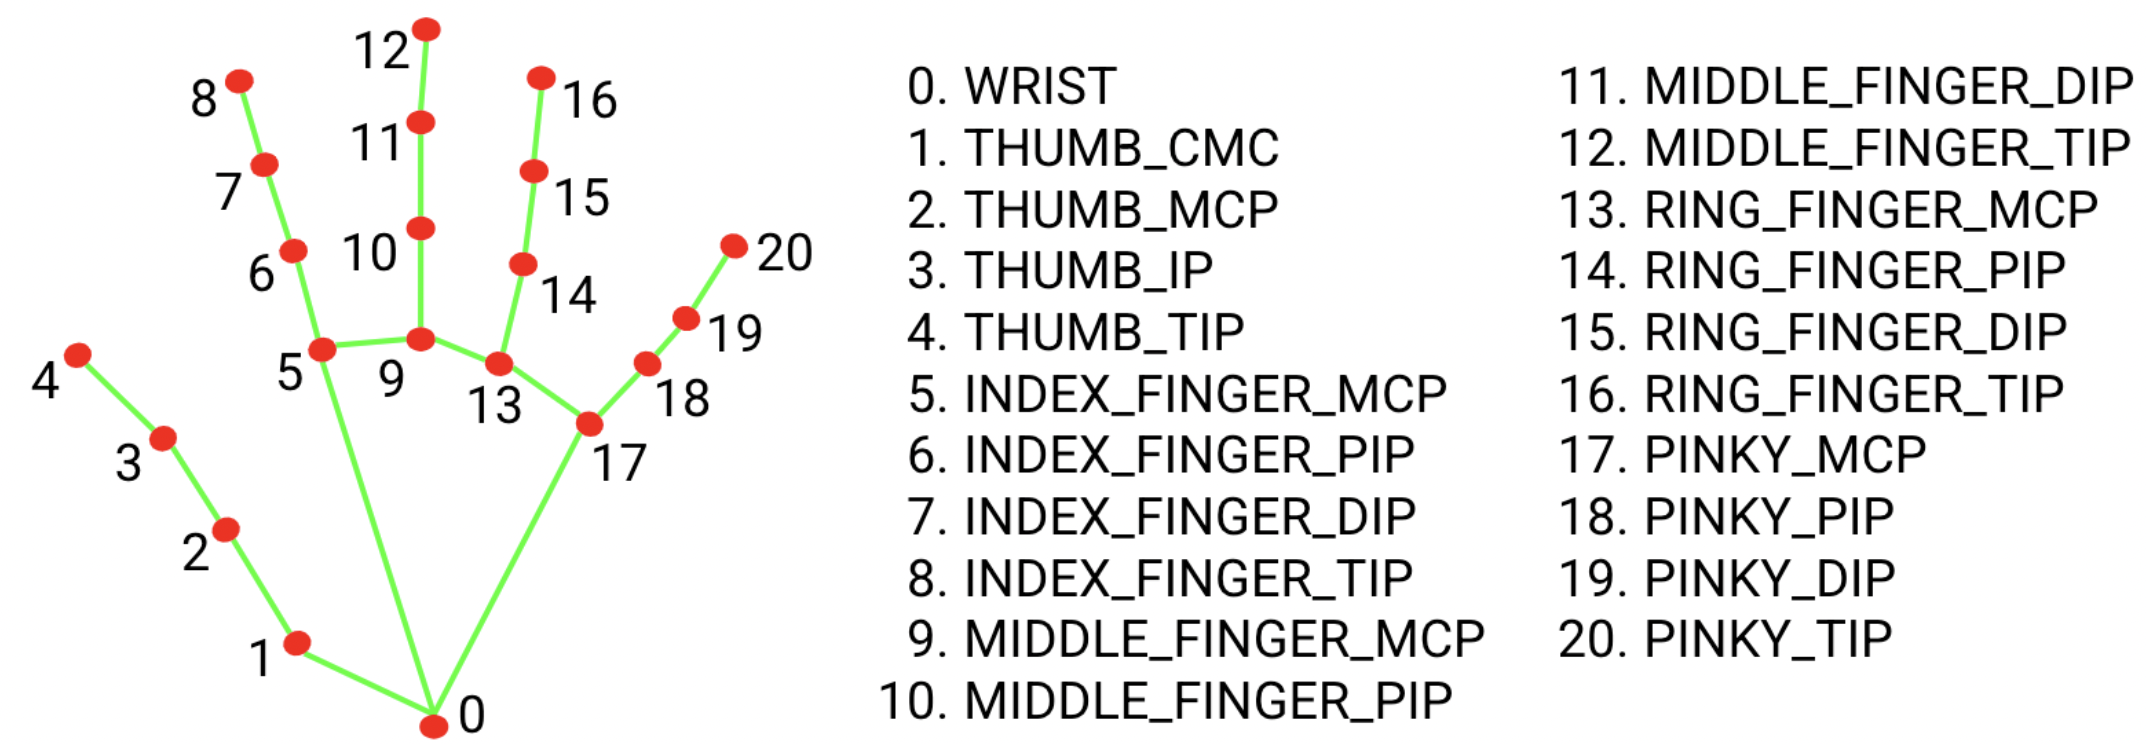
\includegraphics[scale=0.4]{CAPITULOS/capitulo2/hand-landmarks.png}
              \centering
              \caption[Puntos de medipipe ]{Puntos de medipipe Hand Landmarks\cite{ref20}}
              \label{fig:imagen_medipipe_hand}
    \end{figure}

\end{enumerate}




\subsection{Ventajas de MediaPipe Holistic}

\begin{itemize}
\item \textbf{Integración completa:} Combina el seguimiento de rostro, manos y cuerpo en un solo framework, lo que facilita el desarrollo de aplicaciones de LSM.
\item \textbf{Rendimiento en tiempo real:} Permite procesar imágenes en tiempo real, lo que es crucial para la fluidez en la traducción de LSM.
\item \textbf{Eficiencia computacional:} Está optimizado para ejecutarse en dispositivos móviles y de escritorio, con bajo consumo de recursos.
\item \textbf{Robustez:} Funciona en diferentes condiciones de iluminación y con diferentes tipos de cámaras.
\item \textbf{Facilidad de uso:} MediaPipe ofrece APIs fáciles de usar para integrar Holistic en aplicaciones de Python, Android y web.
\end{itemize}

\section{TensorFlow/Keras}
TensorFlow, una plataforma de aprendizaje automático de código abierto, y Keras, una interfaz de alto nivel para construir y entrenar modelos de redes neuronales, son herramientas esenciales en el desarrollo de modelos de aprendizaje profundo. Estos modelos, entrenados con datos de LSM, son capaces de reconocer y clasificar señas, formando la base del sistema de traducción \cite{ref34}.

\section{Procesamiento Híbrido (Local y en la Nube)}
El enfoque híbrido combina el procesamiento local en el dispositivo del usuario con el procesamiento en la nube a través de Amazon Web Services (AWS). Esta estrategia aprovecha las ventajas de ambos entornos: el procesamiento local reduce la latencia y protege la privacidad, aspectos cruciales al tratar con datos sensibles como la comunicación en LSM, mientras que la nube ofrece potencia de cómputo escalable para tareas intensivas, como el entrenamiento de modelos y el almacenamiento de datos \cite{ref35}.

\section{Amazon Web Services (AWS)}
AWS proporciona una amplia gama de servicios en la nube que son fundamentales para el proyecto:
\begin{itemize}
    \item \textbf{Buckets S3:} Almacenamiento escalable y seguro para grandes volúmenes de datos de LSM, como videos y modelos de aprendizaje profundo.
    \item \textbf{Colas SQS:} Facilitan la comunicación asincrónica entre los diferentes microservicios del sistema, permitiendo el procesamiento eficiente y desacoplado de solicitudes de traducción.
    \item \textbf{Funciones Lambda:} Ejecutan código sin necesidad de aprovisionar o administrar servidores, lo que permite escalar automáticamente el procesamiento de solicitudes de traducción según la demanda \cite{ref5}.
\end{itemize}

\section{Lingüística de la Lengua de Señas Mexicana (LSM)}
La LSM, como cualquier lengua natural, posee una gramática compleja que incluye aspectos como la configuración manual, la ubicación, la orientación y el movimiento de las manos, así como las expresiones faciales. El proyecto incorpora conocimientos lingüísticos de la LSM para asegurar una traducción precisa y culturalmente apropiada. La Matriz Segmental, que describe la estructura de las señas en términos de segmentos secuenciales, es una herramienta clave para el análisis y la representación de las señas en el sistema \cite{ref36}.

\subsection{Composición de una seña en la Lengua de Señas Mexicana (LSM)}

La Lengua de Señas Mexicana (LSM), al igual que otras lenguas de señas, se caracteriza por ser una lengua visual-gestual donde la información se transmite a través de la combinación de movimientos y configuraciones de las manos, expresiones faciales y movimientos del cuerpo. Para comprender la estructura de la LSM, es fundamental analizar los elementos que componen una seña.  \cite{ref42}

Una seña en LSM se compone de la articulación simultánea de tres matrices principales:

\subsection{Matriz Segmental:}

Esta matriz se centra en la descripción de la actividad manual,  analizando el movimiento y la detención de la mano.

\begin{itemize}
    \item \textbf{Segmentos:} Se distinguen dos tipos de segmentos:
    \begin{itemize}
        \item \textbf{Movimiento (M):}  Existe un cambio en la configuración o ubicación de la mano en el espacio.
        \item \textbf{Detención (D):} La mano mantiene su posición sin cambios.
    \end{itemize}

    \item \textbf{Tipos de movimiento:}
    \begin{itemize}
        \item \textbf{Movimientos de contorno:}  Describen una trayectoria en el espacio, como lineal, arco, círculo, zigzag, etc.
        \item \textbf{Movimientos locales:} No describen una trayectoria espacial, como movimientos ondulatorios, circulares o de cabeceo.
    \end{itemize}

    \item \textbf{Cualidades de los rasgos:}
    \begin{itemize}
        \item \textbf{Temporal:} Describe la duración del movimiento (sostenido, abreviado, lento, etc.).
        \item \textbf{No temporal:} Describe alteraciones físicas en la ejecución del movimiento (tenso, menguado, ampliado).
        \item \textbf{Contacto:} Describe la relación de proximidad entre la mano y otra parte del cuerpo o el espacio (rozando, rebote).
    \end{itemize}

    \item \textbf{Cualidad espacial:} Describe la orientación de la trayectoria del movimiento en el espacio (plano horizontal, vertical, etc.).
\end{itemize}


\subsection{Matriz Articulatoria:}

Esta matriz describe la postura de la mano en la producción de la seña, considerando diferentes parámetros:

\begin{itemize}
    \item \textbf{Configuración de la mano (CM):} Especifica la forma que adopta la mano, incluyendo la posición de los dedos y el pulgar.  Por ejemplo, mano extendida, mano en puño, dedos flexionados, etc.

    \item \textbf{Ubicación (UB):} Indica el lugar donde se realiza la seña con respecto al cuerpo o el espacio de señalización. Puede ser en la frente, la cabeza, el pecho, el espacio neutro frente al cuerpo, etc.

    \item \textbf{Dirección (DI):} Indica hacia dónde se dirige la palma de la mano durante la ejecución de la seña.  Las opciones incluyen palma arriba, palma abajo, palma hacia el cuerpo, palma hacia afuera, etc.

    \item \textbf{Orientación (OR):} Describe la orientación de la mano con respecto al plano horizontal.  Puede ser con la palma hacia arriba (base), la palma hacia abajo (dorso), o con la palma lateral.
\end{itemize}

\subsection{Matriz de Rasgos No Manuales (RNM):}

Esta matriz se refiere a los elementos no manuales que acompañan la producción de la seña y que contribuyen a su significado.

\begin{itemize}
    \item \textbf{Expresiones faciales:} Incluyen movimientos de las cejas (levantadas, fruncidas), ojos (abiertos, cerrados), nariz (arrugada), boca (sonrisa, labios fruncidos) que modifican la interpretación de la seña.

    \item \textbf{Movimientos de la cabeza:}  Involucran movimientos como el cabeceo (afirmación, negación), la inclinación lateral, o la rotación de la cabeza, que complementan el significado de la seña.

    \item \textbf{Posturas del cuerpo:} Se refiere a la posición general del cuerpo durante la señalización, como la inclinación del torso, los hombros encogidos, etc.
\end{itemize}



\section{ Arquitectura de Microservicios}
El proyecto adopta una arquitectura de microservicios en la parte del entrenamiento del modelo, donde cada componente del sistema se implementa como un servicio independiente y autónomo. Esta modularidad facilita el desarrollo, la implementación y el mantenimiento del sistema, permitiendo escalar y actualizar componentes individuales sin afectar el funcionamiento global \cite{ref37}.

\section{Redes Neuronales}
Las redes neuronales son un conjunto de algoritmos inspirados en la estructura del cerebro humano, diseñados para reconocer patrones. Se componen de nodos interconectados, organizados en capas, que procesan y transmiten información.
\subsection{Redes Neuronales Convolucionales (CNN)}

Las Redes Neuronales Convolucionales (CNN) son una red neuronal profunda con gran eficacia en el procesamiento de imágenes y videos. Esta capacidad se debe a su estructura, enfoca analizar datos organizados en forma de grilla, como es el caso de las imágenes. En el contexto de la traducción de la Lengua de Señas Mexicana (LSM), las CNN tienen un rol fundamental, ya que facilitan el análisis de las imágenes que capturan las señas realizadas por el usuario.

Las CNN se caracterizan por la inclusión de capas convolucionales. Estas capas emplean filtros (kernels), que se deslizan sobre la imagen de entrada para identificar y extraer características relevantes.


\section{Convolución: Definición General}

La convolución  se puede definir como la integral del producto de dos funciones después de desplazar una de ellas una distancia $t$, como se observa en la ecuación \ref{eq:convolucion_continua}:


\indexedequation{Convolucion Definición general}{
    f(x) = \begin{equation}
               S(t) = \int_{-\infty}^{\infty} x(a)w(t-a) da
               \label{eq:convolucion_continua}
    \end{equation}
}



donde:

\begin{itemize}
    \item  $x(a)$ Es la señal de entrada (entrada de la red).
    \item  $w(t-a)$ Es la segunda función (kernel) desplazada una distancia $t$.
    \item  $S(t)$ Es la función resultante de operar la convolución.
\end{itemize}

La salida ($S$) se conoce como mapa de características.


\subsection{Convolución Discreta}

Al tener que procesar datos en una computadora, el tiempo y la señal de entrada se discretizan.  En consecuencia, la operación de convolución se adapta al dominio discreto, como se expresa en la ecuación \ref{eq:convolucion_discreta}:

\indexedequation{Convolucion Discreta}{
    \begin{equation}
        S(t) = (x * w)(t) = \sum_{a = -\infty}^{\infty} x(a)w(t-a)
        \label{eq:convolucion_discreta}
    \end{equation}
}





\subsection{Convolución en 2 Dimensiones}

Las imágenes son datos bidimensionales, por lo que la convolución se extiende a dos dimensiones. Si $I$ representa la imagen de entrada y $K$ representa el kernel, la convolución 2D se define como:

\indexedequation{Convolución en 2 Dimensiones}{
    \begin{equation}
        S(i,j) = (I * K)(i,j) =  \sum_{m} \sum_{n} I(m,n) K(i-m, j-n)
        \label{eq:convolucion_2d}
    \end{equation}
}



donde:

\begin{itemize}
    \item $S(i,j)$ representa el valor del píxel en la posición $(i,j)$ del mapa de características de salida.
    \item $I(m,n)$ representa el valor del píxel en la posición $(m,n)$ de la imagen de entrada.
    \item $K(i-m,j-n)$ representa el valor del elemento en la posición $(i-m,j-n)$ del kernel.
\end{itemize}

\begin{figure}[h]
    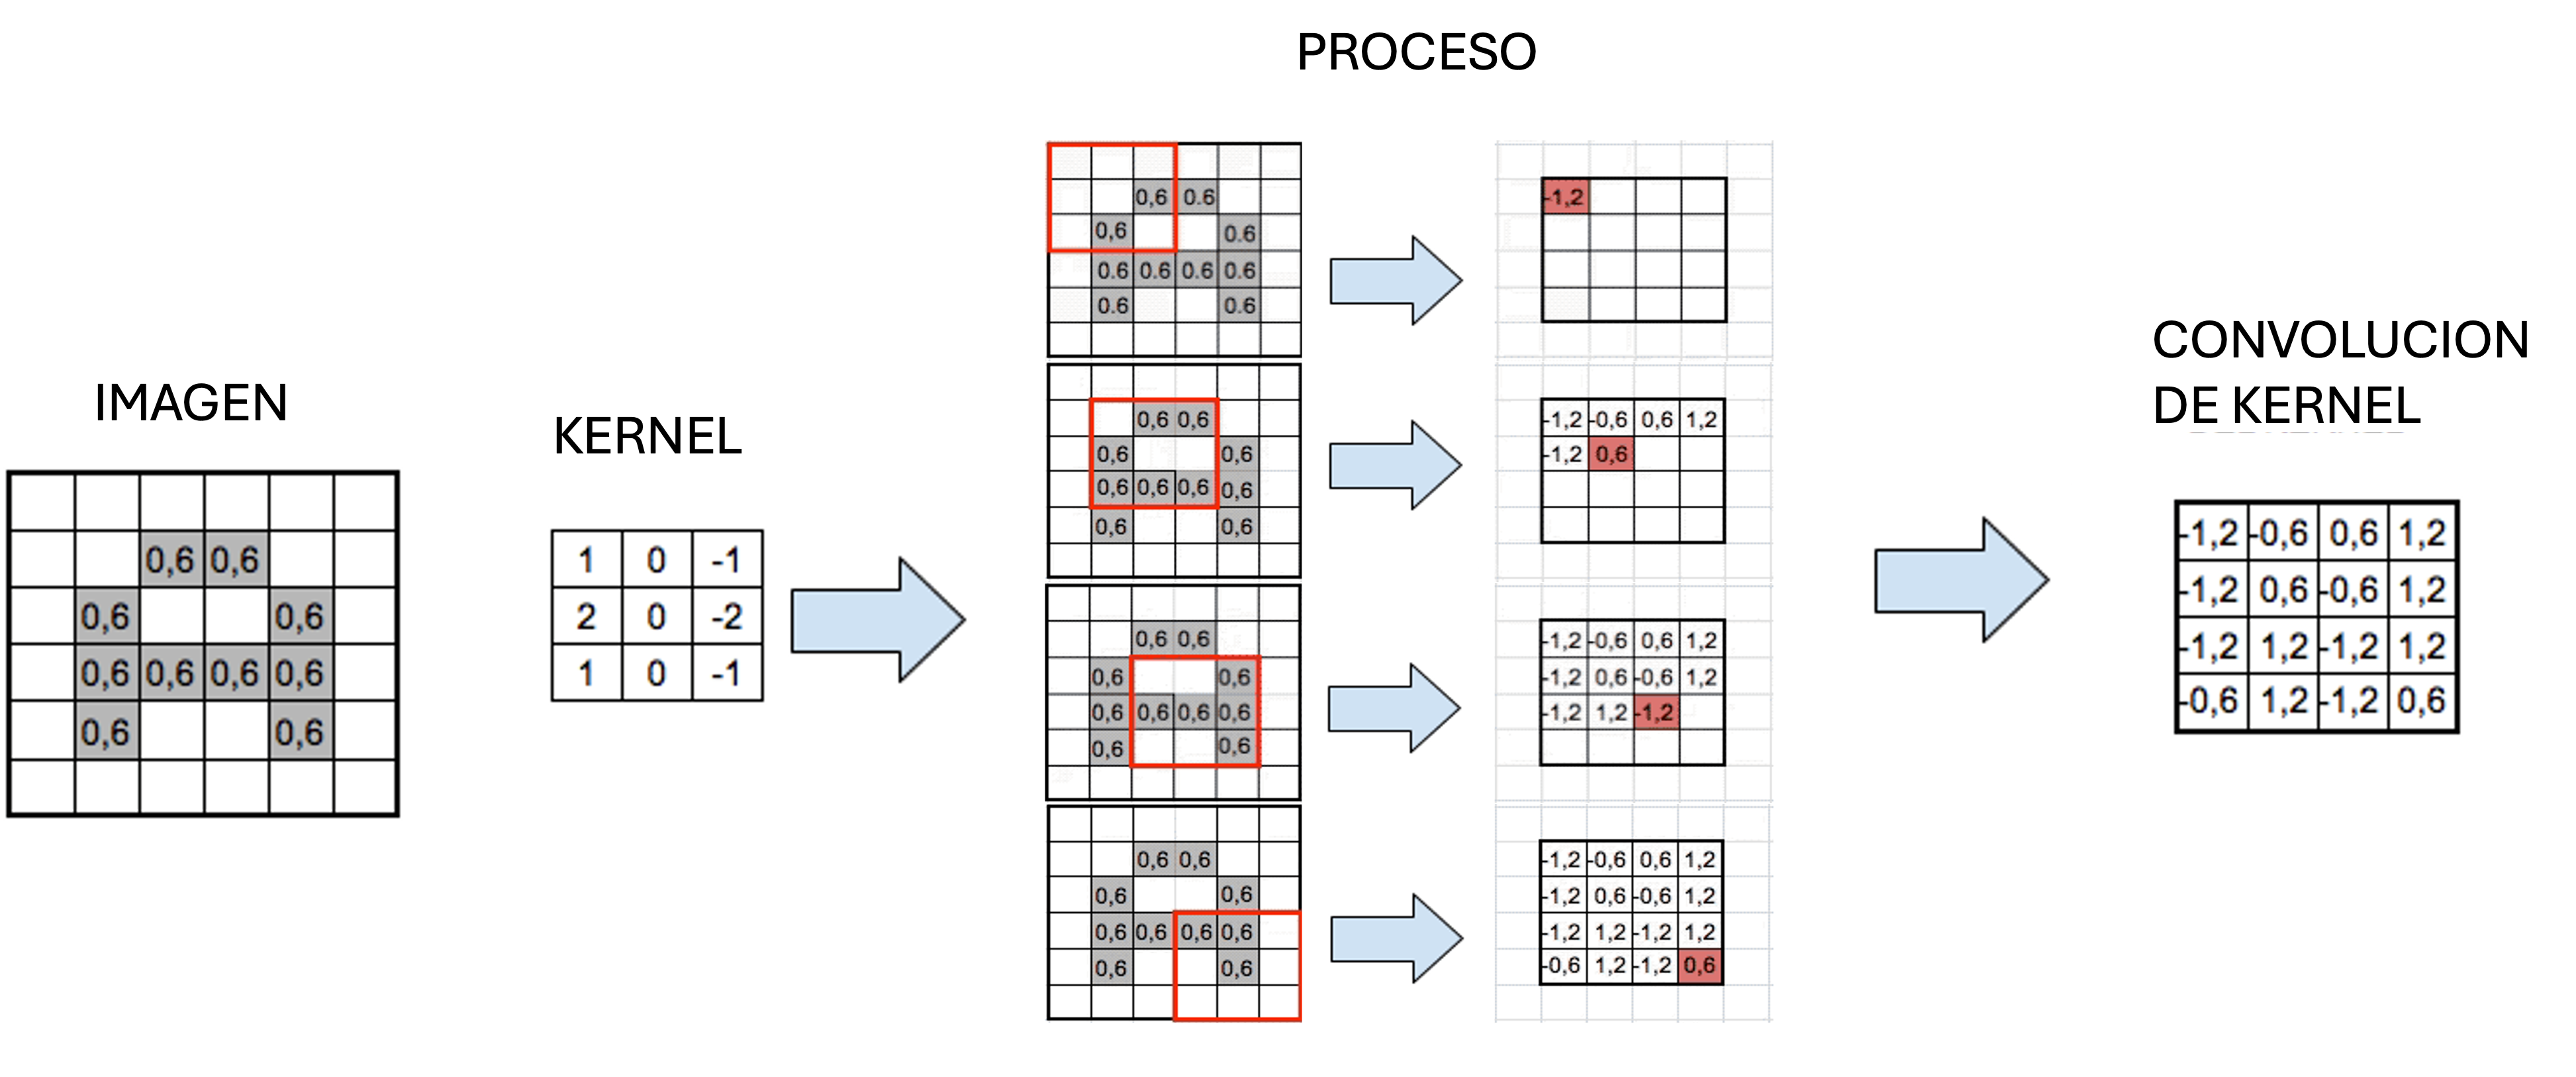
\includegraphics[width=0.9\textwidth]{CAPITULOS/capitulo2/imagenpresentacion}
    \centering
    \caption{Acción de Convolución}
    \label{fig:accion_convolucion}
\end{figure}



De esta manera, se ilustra la transición de la convolución en su forma general a la convolución discreta y, finalmente, a la convolución 2D empleada en las CNN para el procesamiento de imágenes.
\subsection{Redes Neuronales Recurrentes (RNN) para el Análisis de Señas Dinámicas}

Las Redes Neuronales Recurrentes (RNN) constituyen una clase de red neuronal artificial que se caracteriza por sus conexiones recurrentes, lo que les confiere la habilidad de procesar secuencias de datos. Esta propiedad las vuelve especialmente idóneas para el reconocimiento de señas dinámicas en la Lengua de Señas Mexicana (LSM), donde la información temporal es fundamental para la adecuada interpretación del significado. A diferencia de las CNN, que se centran principalmente en el análisis de las características espaciales de las imágenes, las RNN se enfocan en la evolución temporal de las señas, considerando cómo la posición y el movimiento de las manos se modifican a lo largo del tiempo.

\subsubsection{LSTM (Long Short-Term Memory)}

Las LSTM (Long Short-Term Memory) son una variante de las RNN que aborda el problema del desvanecimiento del gradiente, un obstáculo frecuente en el entrenamiento de RNN tradicionales. Este problema dificulta la captura de dependencias a largo plazo en las secuencias de datos. Las LSTM, con su arquitectura de memoria a corto y largo plazo, superan esta limitación y permiten modelar secuencias más extensas y complejas.

\paragraph{Arquitectura de una celda LSTM}

Una celda LSTM está compuesta por tres puertas principales:

\begin{itemize}
    \item \textbf{Puerta de entrada:} Regula la entrada de nueva información a la memoria de la celda.
    \item \textbf{Puerta de olvido:} Determina qué información se descarta de la memoria de la celda.
    \item \textbf{Puerta de salida:}  Controla qué información se utiliza para actualizar el estado oculto de la celda.
\end{itemize}

\paragraph{Ecuaciones de una celda LSTM}

Las siguientes ecuaciones describen el funcionamiento de una celda LSTM:

\begin{align*}
    i_t &= \sigma(W_{xi} x_t + W_{hi} h_{t-1} + b_i) \\
    f_t &= \sigma(W_{xf} x_t + W_{hf} h_{t-1} + b_f) \\
    o_t &= \sigma(W_{xo} x_t + W_{ho} h_{t-1} + b_o) \\
    \tilde{c}_t &= tanh(W_{xc} x_t + W_{hc} h_{t-1} + b_c) \\
    c_t &= f_t * c_{t-1} + i_t * \tilde{c}_t \\
    h_t &= o_t * tanh(c_t)
\end{align*}

donde:

\begin{itemize}
    \item $x_t$: Vector de entrada en el instante $t$.
    \item $h_t$: Estado oculto en el instante $t$.
    \item $c_t$: Estado de la celda en el instante $t$.
    \item $i_t$, $f_t$, $o_t$:  Valores de las puertas de entrada, olvido y salida, respectivamente.
    \item $\tilde{c}_t$:  Candidato al nuevo estado de la celda.
    \item $W_{xi}$, $W_{hi}$, etc.: Matrices de pesos.
    \item $b_i$, $b_f$, etc.: Vectores de sesgo.
    \item $\sigma$: Función sigmoide.
    \item $tanh$: Función tangente hiperbólica.
\end{itemize}

\paragraph{Complemento a la red neuronal convolucional}

En el proyecto de identificación de señas LSM, las LSTM complementan a las CNN al procesar la información temporal de las secuencias de imágenes. Mientras que las CNN extraen características espaciales de cada imagen, las LSTM modelan la evolución de estas características a lo largo del tiempo, capturando la dinámica de las señas. Esta combinación de CNN y LSTM permite un análisis más completo de las señas, mejorando la precisión del sistema de reconocimiento.

En resumen, la incorporación de LSTM en el proyecto de identificación de señas LSM permite un análisis más preciso y robusto de las señas dinámicas, al considerar la información temporal en conjunto con las características espaciales extraídas por las CNN.
\section{Funciones de Activación}
Las funciones de activación introducen no linealidad en las redes neuronales, permitiendo que estas aprendan patrones complejos en los datos. Imaginemos que nuestra red se encuentra ante una bifurcación en el camino; las funciones de activación son responsables de decidir hacia dónde dirigirse.

\subsection{Función Sigmoide}
La función sigmoide transforma cualquier valor de entrada a un rango entre 0 y 1. Esta función es especialmente útil en la capa de salida para problemas de clasificación binaria, como determinar si una seña corresponde a una palabra específica.

\begin{figure}[H]
    \centering
    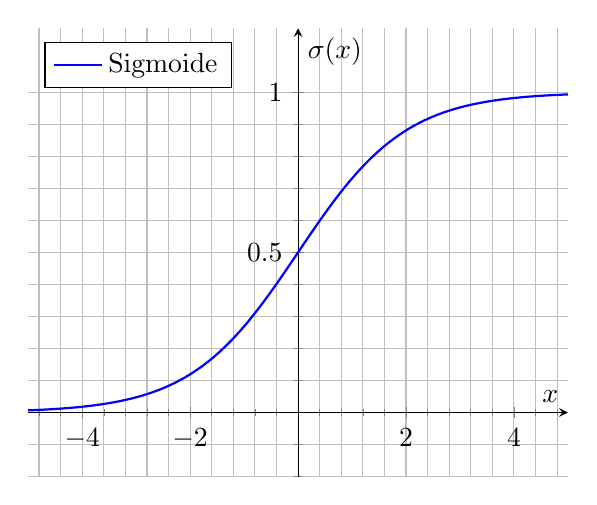
\begin{tikzpicture}
        \begin{axis}[
            xlabel={$x$},
            ylabel={$\sigma(x)$},
            xmin=-5, xmax=5,
            ymin=-0.2, ymax=1.2,
            legend pos=north west,
            axis lines=middle,
            grid=both,
            minor tick num=4,
        ]
        \addplot[domain=-5:5, samples=100, blue, thick] {1/(1+exp(-x))};
        \legend{Sigmoide}
        \end{axis}
    \end{tikzpicture}
    \caption{Gráfica de la función sigmoide.}
\end{figure}

% Función por partes
\indexedequation{Función de activacion Sigmoide}{
f(x) = \begin{cases}
      \frac{1}{1 + e^{-x}}
   \end{cases} \label{eq:funcion_por_partes_sigmoide}
}


\subsection{Función Tangencial Hiperbólica (tanh)}

La función tangencial hiperbólica, conocida como tanh, es otra función de activación que produce valores en el rango de (-1, 1). A diferencia de la sigmoide, que se limita a valores positivos, tanh puede asignar salidas tanto negativas como positivas. Esto la hace especialmente adecuada para problemas donde es necesario identificar tanto clases positivas como negativas, o en situaciones donde se requiere una salida centrada en cero.

\begin{figure}[H]
    \centering
    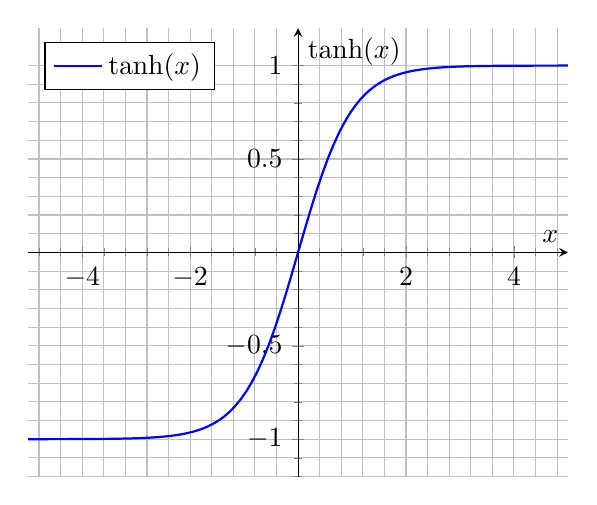
\begin{tikzpicture}
        \begin{axis}[
            xlabel={$x$},
            ylabel={$\tanh(x)$},
            xmin=-5, xmax=5,
            ymin=-1.2, ymax=1.2,
            legend pos=north west,
            axis lines=middle,
            grid=both,
            minor tick num=4,
        ]
        \addplot[domain=-5:5, samples=100, blue, thick] {tanh(x)};
        \legend{$\tanh(x)$}
        \end{axis}
    \end{tikzpicture}
    \caption{Gráfica de la función tangencial hiperbólica ($\tanh$).}
\end{figure}

% Función por partes de tanh
\indexedequation{Función de activacion (tanh)}{
f(x) = \begin{cases}
      -1, & \text{si } x \to -\infty \\
      1, & \text{si } x \to +\infty \\
      \tanh(x), & \text{de otra manera}
   \end{cases} \label{eq:tanh}
}

La función tangencial hiperbólica (tanh), se define mediante la siguiente fórmula:

\indexedequation{Definición tanh}{
\tanh(x) = \frac{e^x - e^{-x}}{e^x + e^{-x}} \label{eq:tanh_formula}
}



\subsection{Función ReLU (Rectified Linear Unit)}
La función ReLU es una función lineal que retorna 0 para entradas negativas y el valor de entrada para entradas positivas. Esta función ha ganado popularidad debido a su simplicidad y eficiencia computacional. En el contexto del reconocimiento de señas, ReLU puede ser utilizada en las capas ocultas de la red neuronal para mejorar la capacidad de aprendizaje del modelo.

\begin{figure}[H]
    \centering
    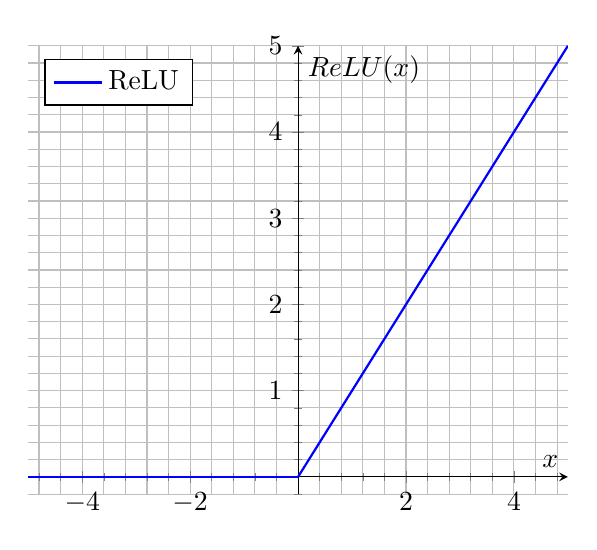
\begin{tikzpicture}
        \begin{axis}[
            xlabel={$x$},
            ylabel={$ReLU(x)$},
            xmin=-5, xmax=5,
            ymin=-0.2, ymax=5,
            legend pos=north west,
            axis lines=middle,
            grid=both,
            minor tick num=4,
        ]
        \addplot[domain=-5:0, samples=100, blue, thick] {0};
        \addplot[domain=0:5, samples=100, blue, thick] {x};
        \legend{ReLU}
        \end{axis}
    \end{tikzpicture}
    \caption{Gráfica de la función ReLU.}
\end{figure}

% Función por partes
\indexedequation{Función de activacion Relu}{
f(x) = \begin{cases}
      0, & \text{si } x < 0 \\
      x, & \text{si } x \geq 0 
   \end{cases} \label{eq:funcion_por_partes_relu}
}

\subsection{Función Softmax}
La función Softmax es frecuentemente utilizada en modelos de clasificación multiclase, ya que convierte las salidas de la red neuronal en probabilidades. Asigna a cada clase una probabilidad que refleja la certeza del modelo sobre su pertenencia, y la clase con la probabilidad más alta se selecciona como la predicción final. Esta función es esencial en muchas redes neuronales profundas, particularmente en la capa de salida de modelos que manejan múltiples categorías.



% Figura para la función Softmax
\begin{figure}[H]
    \centering
    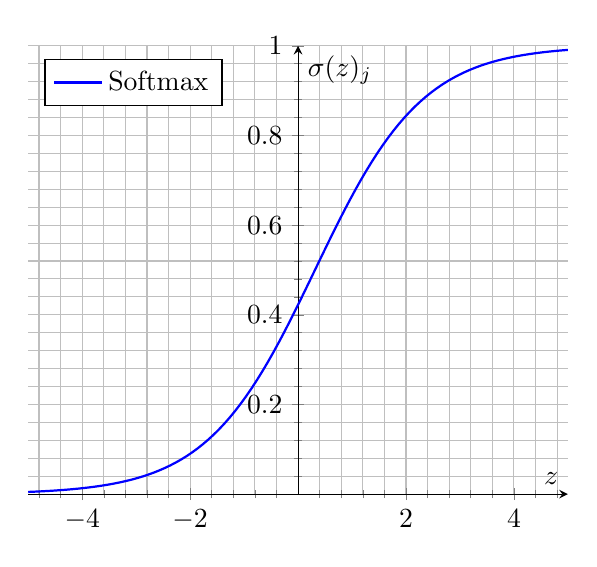
\begin{tikzpicture}
        \begin{axis}[
            xlabel={$z$},
            ylabel={$\sigma(z)_j$},
            xmin=-5, xmax=5,
            ymin=0, ymax=1,
            legend pos=north west,
            axis lines=middle,
            grid=both,
            minor tick num=4
        ]
            % Softmax example with three fixed components
            \addplot[domain=-5:5, samples=100, blue, thick] 
                {exp(x)/(exp(x) + exp(0) + exp(-1))};
            \legend{Softmax}
        \end{axis}
    \end{tikzpicture}
    \caption{Gráfica de la función de activación Softmax considerando tres valores fijos \( z = -1, 0, 1 \).}
    \label{fig:softmax}
\end{figure}

\indexedequation{ Función de activación Softmax}
\sigma(z)_j = \frac{e^{z_j}}{\sum_{k=1}^K e^{z_k}} \label{eq:softmax}
}


Las funciones de activación juegan un papel crucial en la reducción de la complejidad computacional. Esto es particularmente relevante, dado que se ejecutan para cada neurona en la red, para cada muestra y en cada ciclo de entrenamiento. Por ejemplo, con un conjunto de 1500 muestras y 10 características en una red con 4 capas de 64 neuronas cada una, esto puede traducirse en millones de ejecuciones en cada iteración de entrenamiento.

Sin funciones de activación, la red operaría de manera lineal, lo que limitaría su capacidad para aprender patrones complejos. 
La función sigmoide, que limita los valores entre (0, 1), es útil para predecir probabilidades. Por otro lado, la tangente hiperbólica (tanh) ofrece un rango de (-1, 1) y es más efectiva para modelar relaciones donde las entradas negativas deben ser fuertemente negativas y las positivas fuertemente positivas.

La función ReLU, en particular, ha demostrado ser extremadamente eficaz en redes neuronales convolucionales y de aprendizaje profundo, ya que descarta las entradas negativas, lo que simplifica el proceso computacional. Por su parte, la variante Leaky ReLU evita el problema de perder información al permitir que algunos valores negativos pasen con un peso reducido.

Finalmente, la función Softmax permite realizar clasificaciones categóricas multiclase y se aplica en las capas de salida, facilitando la interpretación de las salidas de la red como probabilidades, lo que es fundamental para muchas aplicaciones de inteligencia artificial.


\section{Entrada de Datos al Modelo}

La entrada de datos al modelo de aprendizaje profundo se realiza en forma de arreglos fila o vectores, que representan las características extraídas de las señas capturadas por la cámara. Estos vectores contienen información sobre la seña en cada cuadro de la secuencia, gracias a un enfoque holístico, permitiendo al modelo aprender a reconocer patrones y clasificar las señas\cite{ref38}.

\indexedequation{ Matriz A}{
    A = \begin{pmatrix} a_1 & a_2 & a_3 & \cdots & a_n \end{pmatrix} \label{eq:matrizA}
}

Donde:

\begin{itemize}
    \item $A$ representa el vector de características.
    \item $a_1, a_2, a_3, \ldots, a_n$ son las características individuales extraídas de la seña, como la posición de la mano, la forma de la mano, la orientación, el movimiento, etc.
\end{itemize}

Este enfoque de representación de datos permite que el modelo capture la información espacial y temporal de la seña de manera eficiente, lo que es fundamental para un reconocimiento preciso de la Lengua de Señas Mexicana (LSM).

\section{Datasets para el Reconocimiento de LSM}

El desarrollo de un sistema de traducción de LSM requiere un conjunto de datos robusto y diverso para entrenar y evaluar los modelos de aprendizaje profundo. Estos datasets deben contener imágenes o videos de personas realizando señas en LSM, junto con sus correspondientes traducciones al español.

\subsection{Características de los Datasets}

Los datasets ideales para el reconocimiento de LSM deben cumplir con las siguientes características:

\begin{itemize}
    \item \textbf{Variedad de Señas:} Incluir un amplio repertorio de señas, abarcando el alfabeto, números, palabras comunes, expresiones faciales y gramática de la LSM.
    \item \textbf{Diversidad de Signantes:} Contener muestras de diferentes signantes con variaciones en edad, género, etnia, experiencia en LSM y estilo de señas.
    \item \textbf{Etiquetado Preciso:} Cada muestra debe estar etiquetada correctamente con su correspondiente traducción al español, incluyendo información sobre la seña, significado y contexto gramatical.
    \item \textbf{Tamaño del Dataset:} Un mayor número de muestras generalmente mejora el rendimiento del modelo, permitiendo un aprendizaje más robusto y una mejor generalización.
    \item \textbf{Formato de Datos:} Los datos deben estar en un formato adecuado para el entrenamiento de modelos de aprendizaje profundo, como imágenes, videos o secuencias de datos.
\end{itemize}
